\documentclass[11pt, a4paper, oneside, listof=totoc]{scrartcl}
\usepackage[T1]{fontenc}
\usepackage[utf8]{inputenc}
\usepackage[ngerman, greek, english]{babel}
\usepackage[onehalfspacing]{setspace}
\usepackage{helvet}
\usepackage[a4paper, left=2.5cm, right=2.5cm]{geometry}
\usepackage[
    backend=biber,
    style=authoryear,
    citestyle=authoryear,
    sorting=nyt,
    sortcites=true,
    dashed=false,
    giveninits=false,
    uniquename=true,
    maxbibnames=999,
    url=true
]{biblatex}
\usepackage{csquotes}
\usepackage[hidelinks]{hyperref}
\usepackage{graphicx}
\usepackage{float}
\usepackage{listings}
\usepackage{xcolor}
\usepackage{courier}
\usepackage{needspace}
\usepackage{trace}
\usepackage{longtable}
\usepackage{tabularx}
\usepackage[automark]{scrlayer-scrpage}
\usepackage{microtype}
\usepackage{svg}
\usepackage{xurl}
\usepackage{enumitem}
\usepackage{csquotes}
\usepackage[acronym]{glossaries}
\usepackage{booktabs}
\usepackage{caption}
\usepackage{mfirstuc}
\usepackage{array}
\usepackage{setspace}
\usepackage{substitutefont}

% linting
% chktex-file 1

% show frames in draft
%\usepackage{showframe}

% set language to english
\selectlanguage{english}

% set font to sans-serif
\renewcommand{\familydefault}{\sfdefault}

% set font for Greek
\substitutefont{LGR}{phv}{cmss}    % when LaTeX wants LGR/phv ⇒ use Computer Modern Sans

% bibliography
\addbibresource{jabref-library.bib}

% custom vars
\newcommand{\thesistitle}{Conception, Implementation, and Evaluation of a Highly Scalable and Highly Available Kubernetes-Based SaaS Platform on Kubernetes Control Plane (KCP)}
\newcommand{\sic}{\textnormal{\textit{[sic]}}}
\newcommand{\see}[1]{(see~\autoref{#1}: \textit{\nameref{#1}})}
\newcolumntype{P}[1]{>{\raggedright\arraybackslash}p{#1}}

% URL formatting
\PassOptionsToPackage{hyphens}{url}

% metadata
\title{\thesistitle}
\author{David Linhardt}
\date{\today}

% page style / numbers
\pagestyle{scrheadings}
\cfoot{\thepage} % Page number in center of footer

% glossary
\makeglossaries
\newacronym{k8s}{K8s}{\gls{k8s@gls}}
\newglossaryentry{k8s@gls}{
    name = {Kubernetes},
    description = {Google-born container-orchestrator that underpins your whole platform}
}

\newglossaryentry{admissionWebhook}{
    name = {Admission Webhook},
    description = {external validator/mutator called by the \gls{api} server before objects are stored}
}

\newglossaryentry{etcd}{
    name = {etcd},
    description = {strongly-consistent key-value store that backs both \gls{k8s@gls} and \gls{kcp} metadata}
}

\newglossaryentry{multiTenancy}{
    name = {multi-tenancy},
    description = {many tenants sharing one platform while remaining logically isolated}
}

\newacronym{saas}{SaaS}{\gls{saas@gls}}
\newglossaryentry{saas@gls}{
    name = {Software as a Service},
    description = {single provider-operated codebase served to all customers}
}

\newacronym{kcp}{KCP}{\gls{kcp@gls}}
\newglossaryentry{kcp@gls}{
    name = {Kubernetes Control Plane},
    description = {multi-tenant, horizontally-scalable control-plane project}
}

\newacronym{msp}{MSP}{\gls{msp@gls}}
\newglossaryentry{msp@gls}{
    name = {Managed Service Provider},
    description = {third-party that runs cloud workloads on a customer's behalf}
}

\newacronym{cgroups}{cgroups}{\gls{cgroups@gls}}
\newglossaryentry{cgroups@gls}{
    name = {control groups},
    description = {Linux kernel feature used to cap CPU/-memory per container}
}

\newacronym{hpa}{HPA}{\gls{hpa@gls}}
\newglossaryentry{hpa@gls}{
    name = {Horizontal Pod Autoscaler},
    description = {controller that scales pods based on metrics}
}

\newacronym{rbac}{RBAC}{\gls{rbac@gls}}
\newglossaryentry{rbac@gls}{
    name = {Role-Based Access Control},
    description = {grant permissions via roles and role bindings}
}

\newacronym{abac}{ABAC}{\gls{abac@gls}}
\newglossaryentry{abac@gls}{
    name = {Attribute-Based Access Control},
    description = {policy decisions based on user/resource attributes}
}

\newacronym{sla}{SLA}{\gls{sla@gls}}
\newglossaryentry{sla@gls}{
    name = {Service Level Agreement},
    description = {contractual performance and availability guarantees}
}

\newglossaryentry{namespace}{
    name = {namespace},
    description = {namescope that virtually partitions a cluster in \gls{k8s@gls}}
}

\newglossaryentry{containerization}{
    name = {containerization},
    description = {packaging code and dependencies in \gls{os}-level \glspl{container}}
}

\newglossaryentry{performanceIsolation}{
    name = {performance isolation},
    description = {ensuring one noisy tenant can't violate another's \gls{sla}}
}

\newglossaryentry{microserviceArchitecture}{
    name = {microservice architecture},
    description = {system composed of small, independently deployable services}
}

\newglossaryentry{container}{
    name = {container},
    description = {A lightweight, portable, and isolated runtime environment that packages an application together with its dependencies and configuration. Containers share the host system's kernel but run in separate user spaces, enabling consistent execution across different environments.}
}

\newacronym{api}{API}{Application Programming Interface}
\newacronym{crd}{CRD}{Custom Resource Definition}
\newacronym{url}{URL}{Uniform Resource Locator}
\newacronym{rest}{REST}{Representational State Transfer}
\newacronym{b2b}{B2B}{Business to Business}
\newacronym{b2c}{B2C}{Business to Customer}
\newacronym{os}{OS}{Operating System}

\newacronym{ha}{HA}{high availability}
\newacronym{api}{API}{Application Programming Interface}
\newacronym{crd}{CRD}{Custom Resource Definition}
\newacronym{url}{URL}{Uniform Resource Locator}
\newacronym{rest}{REST}{Representational State Transfer}
\newacronym{b2b}{B2B}{Business to Business}
\newacronym{b2c}{B2C}{Business to Customer}
\newacronym{os}{OS}{Operating System}
\newacronym{sla}{SLA}{Service Level Agreement}
\newacronym{abac}{ABAC}{Attribute-Based Access Control}
\newacronym{rbac}{RBAC}{Role-Based Access Control}
\newacronym{hpa}{HPA}{Horizontal Pod Autoscaler}
\newacronym{cgroups}{cgroups}{control groups}
\newacronym{msp}{MSP}{Managed Service Provider}
\newacronym{kcp}{KCP}{Kubernetes Control Plane}
\newacronym{k8s}{K8s}{Kubernetes}
\newacronym{saas}{SaaS}{Software as a Service}
\newacronym{tcp}{TCP}{Transmission Control Protocol}
\newacronym{ip}{IP}{Internet Protocol}
\newacronym{crud}{CRUD}{Create Read Update Delete}
\newacronym{smb}{SMB}{small and medium sized businesses}
\newacronym{diy}{DIY}{do it yourself}
\newacronym{sql}{SQL}{Structured Query Language}
\newacronym{ttl}{TTL}{time to live}
\newacronym{rpo}{RPO}{recovery point objective}
\newacronym{wal}{WAL}{write-ahead logging}
\newacronym{rto}{RTO}{recovery time objective}
\newacronym{ci}{CI}{continuous integration}
\newacronym{cd}{CD}{continuous deployment}
\newacronym{devops}{DevOps}{development and operations}
\newacronym{io}{I/O}{input / output}
\newacronym{ui}{UI}{user interface}
\newacronym{slo}{SLO}{service-level objective}
\newacronym{qps}{QPS}{queries per second}
\newacronym{cpu}{CPU}{central processing unit}
\newacronym{html}{HTML}{hypertext markup language}
\newacronym{js}{JS}{JavaScript}
\newacronym{ts}{TS}{TypeScript}
\newacronym{ssr}{SSR}{server-side rendering}
\newacronym{db}{DB}{database}
\newacronym{json}{JSON}{JavaScript Object Notation}
\newacronym{fe}{FE}{frontend}
\newacronym{pvc}{PVC}{Persistent Volume Claim}
\newacronym{fs}{FS}{filesystem}
\newacronym{rox}{ROX}{ReadOnlyMany}
\newacronym{pv}{PV}{Persistent Volume}
\newacronym{ssh}{SSH}{Secure Shell}
\newacronym{yaml}{YAML}{YAML Ain't Markup Language, formerly Yet Another Markup Language}
\newacronym{dns}{DNS}{Domain Name System}
\newacronym{sha}{SHA}{Secure Hash Algorithm}
\newacronym{kpi}{KPI}{Key Performance Indicator}
\newacronym{vpa}{VPA}{Vertical Pod Autoscaler}
\newacronym{keda}{KEDA}{Kubernetes Event Driven Autoscaler}
\newacronym{aws}{AWS}{Amazon Web Services}
\newacronym{hnc}{HNC}{Hierarchical Namespace Controller}
\newacronym{eu}{EU}{European Union}
\newacronym{cncf}{CNCF}{Cloud Native Computing Foundation}


\begin{document}

    \newgeometry{top=1cm, bottom=1cm, left=2.5cm, right=2.5cm}

    \begin{titlepage}
        \thispagestyle{empty}

        \hspace*{-1.5cm}
        \noindent
        \hfill
        % THI Logo
        \begin{minipage}{0.3\textwidth}
            \raggedleft\
            \hspace*{1cm}
            
\includegraphics[width=1\textwidth]{images/thi_logo.pdf}
        \end{minipage}

        \vspace{1cm}

        \hrulefill

        \vspace{4cm}

        % header box
        \noindent
        \makebox[\textwidth][c]{
            \parbox{10cm}{
                \LARGE\textbf{Technische Hochschule Ingolstadt}\\
                \\
                \Large\textbf{Specialist area Computer Science}\\
                \Large\textbf{Bachelor's course Computer Science}\\
            }
        }

        % bachelors thesis
        \begin{center}
            \LARGE\textbf{Bachelor's thesis}
        \end{center}

        \vspace{1cm}

        % tabularx
        \begin{tabularx}{\textwidth}{@{}lX@{}}
            \textbf{Subject:} & \thesistitle\\[2cm]
            \textbf{Name and Surname:} & David Linhardt \\[0.5cm]
            \textbf{Matriculation number:} & 00122706\\[2cm]     
            \textbf{Issued on:} & 2025--04--09 \\[0.5cm]           
            \textbf{Submitted on:} & 2025--08--01 \\[2cm]           
            \textbf{First examiner:} & Prof.\ Dr.\ Bernd Hafenrichter \\[0.5cm]      
            \textbf{Second examiner:} & Prof.\ Dr.\ Ludwig Lausser \\
        \end{tabularx}

    \end{titlepage}

    \begin{titlepage}
        \hspace*{-1.5cm}
        \noindent
        \hfill
        % THI Logo
        \begin{minipage}{0.3\textwidth}
            \raggedleft\
            \hspace*{1cm}
            
\includegraphics[width=1\textwidth]{images/thi_logo.pdf}
        \end{minipage}

        \vspace{1cm}

        \LARGE\textbf{Declaration in Accordance with §~30~Abs.~4~Nr.~7~APO~THI}\\

        \vspace{1cm}

        \hrulefill

        \vspace{2cm}
        
        \begin{center}
            \LARGE\textbf{Declaration}\\
        \end{center}
        \vspace{1cm}
        \normalsize
        I hereby declare that this thesis is my own work, that I have not presented it elsewhere for
        examination purposes and that I have not used any sources or aids other than those stated.
        I have marked verbatim and indirect quotations as such.\\[1cm]
        Ingolstadt, 2025--08--01\\[2cm]
        David Linhardt

    \end{titlepage}

    \restoregeometry

    \pagenumbering{roman}

    \section*{Abstract}\label{abstract}
    \markboth{Abstract}{Abstract}

    \newpage

    % Glossary
    \printglossary[type=\acronymtype, title={Acronyms}]
    \cleardoublepage
    \printglossary[title={Glossary}]


    \cleardoublepage

    % TOC
    \begingroup
        \microtypesetup{protrusion=false}
        \tableofcontents
    \endgroup

    \newpage

    \cleardoublepage
    \begingroup
        \renewcommand{\addcontentsline}[3]{}
        \listoffigures
    \endgroup

    \cleardoublepage
    \begingroup
        \renewcommand{\addcontentsline}[3]{}
        \listoftables
    \endgroup

    \newpage

    \pagenumbering{arabic}

    \section{Introduction}\label{sec:introduction}

        \subsection{Problem Statement and Motivation}\label{subsec:problem}

        \subsection{Objectives and Scope}\label{subsec:objectives}

        \subsection{Structure of the Thesis}\label{subsec:structure}

    \section{Fundamentals}

        \subsection{Kubernetes and Multi-Tenancy}\label{subsec:k8sAndMultiTenancy}

            \subsubsection{Kubernetes as the Foundation for Cloud-Native Applications}\label{subsubsec:foundationK8s}
                As the de facto standard for deploying and managing 
                \textit{cloud-native applications}, \gls{k8s@gls}, commonly referred to as \gls{k8s}
                plays a pivotal role in modern cloud architecture \parencite[p.~7--8]{poulton2021}.
                \gls{k8s@gls} works as an  orchestrator for \textit{containerized,
                cloud-native microservice} applications, meaning it can deploy apps and dynamically
                respond to changes \parencite[p.~3]{poulton2021}.
                It offers a platform for declarative configuration and automation for containerized
                workloads, enabling organizations to run distributed applications and services at
                scale \parencite{kubernetesOverview,redhatWhatIsKubernetes}.

            \subsubsection{The Importance of Multi-Tenancy in Modern SaaS Platforms}\label{subsubsec:mtImportance}
                Multi-tenancy plays a fundamental role in modern cloud computing.
                By allowing multiple tenants to share the same infrastructure through
                virtualization, it significantly increases resource utilization, reduces operational
                costs, and enables essential features such as VM mobility and dynamic resource
                allocation \parencite[pp.~345--346]{aljahdali2014}. 
                These benefits are crucial for cloud providers, as they make the cloud business
                model economically viable and scalable.
                In the context of modern \gls{saas} platforms, \gls{multiTenancy} goes even further
                by enabling unified management, frictionless onboarding, and simplified operational
                processes that allow providers to add new tenants without introducing incremental
                complexity or cost \parencite[pp.~9--11]{awsSaaSArchitectureFundamentals}.
                \\
                However, while \gls{multiTenancy} is indispensable for achieving efficiency,
                scalability, and cost-effectiveness, it simultaneously introduces complex security
                challenges, especially in shared environments where resource isolation is limited. 
                In particular, the potential for cross-tenant access and side-channel attacks makes
                security in multi-tenant environments a primary concern
                \parencite[pp.~345--346]{aljahdali2014}. 
                As such, understanding and addressing \gls{multiTenancy} from both operational and
                security perspectives is essential when designing and securing modern cloud-native
                platforms
                \parencites[pp.~9--11]{awsSaaSArchitectureFundamentals}[p.~4]{isoConcepts}.

            \subsubsection{The Challenges of Multi-Tenancy and the Need for Solutions}\label{subsubsec:challenges}
                Multi-tenancy introduces a spectrum of technical and security challenges that need
                to be addressed.

                \begin{enumerate}[label={[\arabic*]:},
                    ref=Challenge~\arabic*,
                    leftmargin=*,
                    itemsep=0.6\baselineskip]

                    \item\label{chal:remanence}
                        \textit{Residual-data exposure}.
                        Shared infrastructures may expose tenants to data leakage and hardware-layer
                        attacks. 
                        Because hardware resources are only virtually partitioned,
                        residual data left in reusable memory or storage blocks,
                        known as \textit{data remanence},
                        can be inadvertently leaked or deliberately harvested by co-resident tenants
                        \parencites[p.~586]{zissis2012}[pp.~344--345]{aljahdali2014}.

                    \item\label{chal:transparency}
                        \textit{Control and transparency}.
                        By design, \gls{saas} moves both data storage and security controls out of
                        the enterprise's boundary and into the provider's multi-tenant cloud,
                        depriving organizations of direct oversight and assurance and thereby
                        heightening concern over how their critical information is protected,
                        replicated and kept available \parencite[pp.~3--4]{subashini2011}.
                        To complicate matters further, the customer might have no way to evaluate
                        the \gls{saas} vendors security measures, meaning the pricing and feature
                        set will most likely determine which service is used in practice, often
                        disregarding security concerns
                        \parencites[p.~6]{everett2009}[p.~836]{khorshed2012}.

                    \item\label{chal:scheduling}
                        \textit{Scheduling}.
                        In multi-tenant architectures multiple tenants utilize the same hardware,
                        thus creating the need for fair scheduling to ensure cost-effectiveness
                        and performance \parencite[p.~32597]{simi2024}.
                        Achieving fair and efficient resource allocation in scheduling first
                        requires a quantitative assessment of the system's existing unfairness
                        \parencites[p.~7]{ebrahimi2012}[p.~14]{beltre2019}[pp.~2--3]{ghodsi2011}.
                        Various scheduling algorithms and policies can be employed in practice to
                        achieve fairness \parencites[pp.~14--16]{beltre2019}[p.~4]{ghodsi2011}.
                        To fully leverage the advantages of multi-tenant architectures, resources
                        must not only be shared fairly, but also efficiently, not hindering
                        performance \parencite[p.~14]{beltre2019}.
                        As stated by~\cite[p.~14]{beltre2019} \enquote{Balancing both cluster
                        utilization and fairness is challenging}.
                    
                    \item\label{chal:isolation}
                        \textit{Performance Isolation}.
                        A single tenant is able to significantly degrade the performance of other
                        tenants working on the same hardware, if \textit{\gls{performanceIsolation}}
                        is not given \parencite[p.~195]{krebs2013}.
                        The fundamental performance expectations of a system are commonly formalized
                        in a \acrfull{sla}.\@ % manual acrfull bcs of gls in glossary
                        As noted by~\cite[p.~195]{krebs2013} \enquote{A system is said to be
                        performance isolated, if for tenants working within their quotas the
                        performance is within the (response time) \gls{sla} while other
                        tenants exceed their quotas (e.g., request rate)}.
                        As noted by~\cite[p.~18]{carrion2022} \enquote{Currently, it is difficult
                        to achieve \gls{performanceIsolation} for \gls{multiTenancy} on \gls{k8s}
                        clusters because this requires providing resource isolation and improving
                        the abstraction of applications.}

                    \item\label{chal:automation}
                        \textit{Automation}.
                        As noted by~\cite[p.~651]{nguyen2022} \enquote{Presently, multi-tenant
                        systems lack the facility of allowing clients to dynamic~\sic
                        change their resources based on their business demands or create and
                        allocate resources for new tenants.
                        Multi-tenant system~\sic administrator manually does all the work of
                        allocation or changing tenant's~\sic resources.}
                        However, to ensure efficiency and scalability, an \gls{api} that allows
                        automating deployments and dynamic changes in the application is needed.

                \end{enumerate}

                A secure solution, keeping multi-tenancies advantages while also addressing security
                concerns is desperately needed
                \parencites[p.~346]{aljahdali2014}[pp.~14576--14577]{senel2023}.

            \subsubsection{Kubernetes Control Plane (KCP) as a Promising Approach}\label{subsubsec:kcpApproach}
                \acrfull{kcp} offers three capabilities that map accurately onto today's
                \gls{multiTenancy} pain points.% manual acrfull bcs glossary

                \begin{enumerate}[label={[\arabic*]:},
                    ref=Challenge~\arabic*,
                    leftmargin=*,
                    itemsep=0.6\baselineskip]

                    \item\label{chal:workspaces}
                        \textit{Workspaces}.
                        \gls{kcp} achieves strong resource isolation through the concept of
                        \textit{workspaces} \see{subsubsec:workspaces}.

                    \item\label{chal:api}
                        \textit{API}.
                        \gls{kcp} offers an \gls{k8s@gls}-like \gls{api} that enables the use of
                        standard tools and automation to a degree \see{subsubsec:api}.
                    
                    \item\label{chal:sharding}
                        \textit{Sharding}.
                        \gls{kcp} offers sharding out of the box to manage high traffic and 
                        geo-distribution \see{subsubsec:sharding}.
                \end{enumerate}

            \subsubsection{Background: The Evolution of Kubernetes}\label{subsubsec:k8sEvolution}
                \gls{k8s@gls}, an open-source \gls{container} orchestration platform developed by
                Google, emerged from the need to manage the complexities of containerized
                applications effectively and to support large-scale deployments in a cloud-native
                environment \parencites{googlecloudWhatIsKubernetes}{kubernetesOverview}.
                It was originally developed at Google and released as open source in 2014
                \parencite{googlecloudWhatIsKubernetes}.
                \gls{k8s@gls} was conceived as a successor to Google's internal \gls{container}
                management system called Borg, and designed to streamline the process of deploying,
                scaling, and managing applications composed of microservices running in containers
                \parencites[pp.~13--14]{verma2015}[p.~84]{bernstein2014}.
                The name \gls{k8s@gls} originates from the Greek word \textgreek{κυβερνήτης} meaning
                helmsman or pilot \parencite{kubernetesOverview}.
                The abbreviation \gls{k8s} results from counting the eight letters in between the
                \enquote{K} and the \enquote{s} \parencite{kubernetesOverview}.
                \\
                Since its inception, \gls{k8s@gls} has gained traction among organizations because it
                provides robust features such as automated scaling,
                self-healing, and service discovery, which have made it the de facto standard for
                \gls{container} orchestration in the tech industry
                \parencite[pp.~855--858]{damarapati2025}.
                \\
                As noted by~\cite[p.~457]{moravcik2022} almost 90\% of organizations used
                \gls{k8s@gls} as an orchestrator for managing containers and over 70\% of organizations
                used it in production by 2021 \parencite{redhatStateOfK8sSecurityReport2021}.
                The widespread adoption of \gls{k8s@gls} is further underscored by Red Hat's latest
                (2024) report, which no longer asks survey respondents if they use \gls{k8s@gls} for
                \gls{container} orchestration, but rather \textbf{which} \gls{k8s@gls} platform they use
                \parencite[p.~27]{redhatStateOfK8sSecurityReport2024}.
                According to~\cite[pp.~855--856]{damarapati2025}, \gls{k8s@gls} has seen
                unprecedented industry adoption due to its vendor neutrality, strong community
                support, and flexible, extensible architecture in combination with readiness for
                enterprise use caused by \gls{ha@gls}, disaster recovery and security.
                \\
                Moreover \gls{k8s@gls} enables faster time-to-market by providing a unified,
                declarative control plane that abstracts away infrastructure,
                guarantees consistent environments from development to production,
                and automates operational tasks such as scaling, rolling updates,
                and self-healing—advantages that translate directly into competitive delivery speed,
                increasing its appeal to organizations of every size
                \parencite[pp.~858--859]{damarapati2025}.
                \\
                Over the years, Kubernetes --- and the many orchestration solutions inspired by or
                built on it --- has evolved to handle an increasingly diverse range of workloads,
                supporting everything from conventional applications in to emerging
                \textit{edge-native} deployments \parencites[p.~21]{biot2025}[pp.~1--4]{biot2025}.
                Edge-native deployments are applications intended to run on computing
                resources located at or near the data source --- the network \textit{edge} ---
                rather than in a central cloud \parencite[p.~34]{satyanarayanan2019}.
                This adaptability reflects its fundamental design, which focuses on modularity and
                extensibility, allowing developers to customize their orchestration needs.
                \\
                Overall, the history of \gls{k8s@gls} showcases a transformative journey driven by the
                evolving demands of software architecture and the necessity for efficient
                application management in an increasingly complex technological landscape.

            \subsubsection{Background: Containerization as an Enabler of Kubernetes}\label{subsubsec:containerization}
                \textit{\Gls{containerization}} is a way to bundle an application's code with all its
                dependencies to run on any infrastructure thus enhancing portability
                \parencite{awsWhatIsContainerization,dockerWhatContainer}.
                The lightweight nature and isolation of \glspl{container} can be leveraged by
                cloud-native software to enable both vertical and horizontal autoscaling,
                facilitated by fast startup times, as well as self-healing mechanisms and support
                for distributed, resilient infrastructures
                \parencites{kubernetesAutoscalingWorkloads}{kubernetesSelfHealing}
                    {awsWhatIsContainerization}[pp.~58--59]{davis2019}.
                Furthermore it complements the microservice architectural pattern by enabling
                isolated, low overhead deployments, ensuring consistent environments
                \parencite[p.~209]{balalaie2016}.

            \subsubsection{Background: The Role of Microservices in Cloud-Native Architectures}\label{subsubsec:microservices}
                \textit{Microservices} play a pivotal role in cloud-native architectures by
                promoting business agility, scalability, and maintainability of applications.
                By decomposing applications into independent, granular services, microservices
                facilitate development, testing, and deployment using diverse technology stacks,
                enhancing interoperability across platforms
                \parencites[p.~1]{waseem2020}[p.~1]{larrucea2018}.
                Additionally, they help prevent failures in one component from propagating across
                the system by isolating functionality into distinct, self-contained services
                \parencite[p.~62]{davis2019}.
                This architectural style aligns well with cloud environments, as it allows services
                to evolve independently, effectively addressing challenges associated with scaling
                and maintenance without being tied to a singular technological framework
                \parencite[pp.~202--203]{balalaie2016}.
                Furthermore, the integration of microservices with platforms like \gls{k8s@gls}
                enhances deployment automation and orchestration, thus providing substantial
                elasticity to accommodate fluctuating workloads \parencite[p.~170]{haugeland2021}.
                Additionally, migrating legacy applications to microservices can foster
                modernization and efficiency, thus positioning organizations favorably in
                competitive landscapes \parencite[p.~214]{balalaie2016}.
                Overall, the synergy between microservices and cloud-native architectures stems from
                their inherent capability to optimize resource utilization and streamline continuous
                integration and deployment processes.

            \subsubsection{Background: Kubernetes Resource Isolation Mechanisms}\label{subsubsec:k8sResourceIsolation}
                \gls{k8s@gls} employs several resource isolation mechanisms, primarily through the
                use of \textit{\gls{cgroups}} and \textit{namespaces} to limit
                resource allocation for containers.
                \Gls{cgroups} are a Linux kernel feature that organizes processes into hierarchical
                groups for fine-grained resource limitation and monitoring via a pseudo-filesystem
                called \textit{cgroupfs} \parencites{kubernetesCgroupsV2}{cgroups7}.
                \textit{Namespaces} are a mechanism for isolating groups of resources within a
                single cluster and scoping resource names to prevent naming conflicts across
                different teams or projects \parencite{kubernetesNamespaces}.
                However, these mechanisms may not always provide the sufficient isolation needed for
                multi-tenant architectures, because the logical segregation offered by namespaces
                does not address the fundamental security concerns associated with
                \gls{multiTenancy} \parencite[p.~651]{nguyen2022}.
                Additionally, research indicates that the native isolation strategies can lead to
                performance interference, where containers that share nodes can experience
                significant degradation in performance due to CPU contention
                \parencite[p.~158]{kim2021}.
                Specifically, critical services may be adversely affected when non-critical services
                monopolize available resources, which undermines the quality of service in
                multi-tenant environments \parencite[p.~30410]{li2019}.
                \\
                Moreover, while \gls{k8s@gls} allows for \gls{container} orchestration and resource
                scheduling, it can lead to resource fragmentation, further exacerbating the issue
                of \gls{performanceIsolation} \parencite[p.~1]{jian2023}.
                A common approach in multi-tenant scenarios is to deploy separate clusters for each
                tenant, which incurs substantial overhead—particularly in environments utilizing
                virtual machines for isolation \parencite[pp.~144574--144575]{senel2023}.
                In summary, although \gls{k8s@gls} offers essential isolation mechanisms, the
                complexities of resource sharing and performance consistency in multi-tenant
                applications highlight the need for enhanced strategies to ensure robust resource
                management and \gls{performanceIsolation}
                \parencites[p.~651]{nguyen2022}[p.~2]{jian2023}[p.~158]{kim2021}.

            \subsubsection{Relevance to SaaS and this Thesis}

        \newpage

        \subsection{Kubernetes Control Plane (KCP)}\label{subsec:kcp}
            \gls{kcp} is \enquote{An open source horizontally scalable control plane for
            \gls{k8s@gls}-like APIs} \parencite{kcpio}.
            % nguyen 2022
            % KCP docs

            \subsubsection{Workspaces}\label{subsubsec:workspaces}
                \gls{kcp} introduces the concept of \textit{workspaces} to implement
                \gls{multiTenancy}.
                In \gls{kcp}, a workspace is a \gls{k8s@gls}-cluster-like HTTPS endpoint exposed
                under \texttt{/clusters/<parent>:<name>}, that regular tools such as
                \textit{kubectl}, \textit{Helm} or \textit{client-go} treat exactly like a real
                \gls{k8s@gls} cluster.
                Every workspace is backed by its own logical cluster stored in an isolated
                \textbf{\gls{etcd} prefix}, so objects in one workspace (including cluster-scoped
                resources like \textbf{CRDs}) are completely invisible to others, delivering hard
                \gls{multiTenancy} without spinning up separate control planes
                \parencite{kcpWorkspaces}.
                \\
                As per the definition by the~\cite{etcd}, \enquote{\textbf{\gls{etcd}} is a strongly
                consistent, distributed key-value store that provides a reliable way to store data
                that needs to be accessed by a distributed system or cluster of machines.
                It gracefully handles leader elections during network partitions and can tolerate
                machine failure, even in the leader node.}
                \gls{etcd} is the primary datastore used by \gls{kcp} and \gls{k8s}
                \parencites{kcpDevStorageToRest}[p.~214]{sun2021}.
                \textbf{\gls{etcd} prefixes} are a simple, inbuilt way to group keys using a prefix
                \parencite{etcdPrefix}.
                This allows for resource isolation in \gls{kcp}.\@
                A \gls{crd} is a declaratively specified schema that registers a new  resource,
                defined by its group, version, kind, and OpenAPI schema, into the \gls{kcp@gls} so
                the native \gls{api} server stores and serves the objects as first-class
                resources \parencite{kubernetesCRD}.
                \\
                \gls{kcp} implements the same \gls{rbac}-based authorization mechanism and cluster
                role and cluster role binding principles as \gls{k8s@gls} inside workspaces 
                \parencite{kcpAuthorization}.
                However unlike \gls{k8s@gls} \gls{kcp} does currently not support \gls{abac}
                \parencites{kcpAuthorization}{kubernetesABAC}.
                \gls{kcp} likely supports only \gls{rbac}-based authorization because \gls{abac} is
                considered overly complex, hard to audit, and increasingly deprecated in favor of
                \gls{rbac}, which offers a more structured and maintainable access control model
                \parencite{kubernetesRBACBlog}.
                This allows for consistent access control and permission management across all
                workspaces, aligning with familiar \gls{k8s@gls} patterns and simplifying
                multi-tenant environment administration.
                \\
                Workspaces allow for a typed, parent-child tree, and each type can constrain which
                kind of workspaces it can contain or be contained by, giving platform teams a
                structured way to delegate environments while retaining policy control
                \parencite{kcpWorkspaces}.
                \\
                This combination of strong isolation, familiar tooling, and hierarchical
                organization makes workspaces offer an attractive solution to many of the problems
                commonly faced in multi-tenant environments: each tenant gets the freedom of a full
                dedicated cluster, yet operators manage only a single shared \gls{kcp} control
                plane.
            
            \subsubsection{API}\label{subsubsec:api}
                As previously noted, most \gls{k8s@gls} based multi-tenant systems currently require
                manual intervention by an administrator to deploy new tenants or modify resource
                allocation.
                However \gls{kcp}, other than similar frameworks, like Capsule or Kiosk, provides an
                \gls{api} server to the customer, that provides an easy way to access
                their resources \parencites[p.~651]{nguyen2022}{kcpio}.
                This in turn enables a degree of automation \parencite[p.~651]{nguyen2022}.
                Every workspace has its own \gls{api} endpoint \parencite{kcpWorkspaces}.
                This ensures, that more control can be shifted back to the customer.
                \gls{kcp} ships a curated set of built-in \gls{k8s@gls} \glspl{api}, such as
                \texttt{Namespaces}, \texttt{ConfigMaps}, \texttt{Secrets} and \gls{rbac} objects, 
                so tenants can start working with familiar primitives immediately
                \parencite{kcpAPIsBuiltIn}.
                Additional functionality can be added per workspace simply by installing a
                \gls{crd}, and \gls{kcp} permits multiple independent versions of the same \gls{crd}
                to coexist across workspaces \parencite{kcpAPIs}.
                \\
                To share an \gls{api} with other tenants, a provider declares an
                \texttt{APIResourceSchema} and then exports it through an \texttt{APIExport},
                while consumers attach that \gls{api} to their workspace with an \texttt{APIBinding}
                \parencite{kcpAPIsExport}.
                This export/bind workflow lets platform teams evolve \glspl{api} centrally without
                touching each consumer workspace, reinforcing the system's self-service goal
                \parencite{kcpAPIsExport}.
                \\
                \gls{kcp} supports \glspl{admissionWebhook} only through \gls{url}-based client
                configurations, while \texttt{service}-based webhooks and conversion webhooks are
                currently unsupported, so operators must host their hooks externally
                \parencite{kcpAPIsAdmissionWebhooks}.
                \\
                Because admission requests include the logical-cluster name, webhook back ends can
                enforce policies per workspace and thus maintain strong tenant isolation
                \parencite{kcpAuthorization}.
                Every \gls{rest} call is scoped under the path pattern
                \texttt{/clusters/<workspace>}, ensuring that automation never leaks objects across
                workspaces \parencite{kcpAPIsREST}.
                \gls{api} providers can also access consumer data through a virtual-workspace
                \gls{url} rooted at \texttt{/services/apiexport/…}, enabling safe cross-workspace
                reconciliation loops without cluster-wide privileges \parencite{kcpAPIsREST}.
                Together, built-in \glspl{api}, \glspl{crd}, the \gls{api}Export / \gls{api}Binding
                model, admission controls and workspace-prefixed \gls{rest} routing give tenants a
                rich yet safe surface for automation while keeping operational responsibility with
                the platform team.

            \subsubsection{Sharding}\label{subsubsec:sharding}
                \gls{kcp} employs sharding to \textbf{horizontally scale} the control-plane, letting
                an installation grow far beyond the limits of a single \gls{api}-server/\gls{etcd}
                pair \parencite{kcpSharding,kcpShardingShards}.
                \\
                Each shard hosts a set of logical clusters, so every workspace (and therefore every
                tenant) gets its own \gls{k8s@gls}-compatible consistency domain on that shard
                \parencite{kcpShardingShards}.
                Because \enquote{a set of known shards comprises a \gls{kcp} installation},
                operators can add or remove shards at will, expanding or contracting capacity with
                no downtime for existing workspaces \parencite{kcpShardingShards}.
                \\
                Cross-shard traffic is funneled through a dedicated \textbf{cache-server}, avoiding
                the \( n \times (n - 1) \) explosion of of direct links that would otherwise appear
                in large deployments \parencite{kcpShardingCacheServer}.
                This cache-server also underpins \textbf{workspace migration and object
                replication}, so tenants remain oblivious to topology changes while the platform
                evolves underneath them \parencite{kcpShardingCacheServer}.
                \\
                Administrators can define \textbf{Partitions} that group shards, for example by
                region or load profile, giving schedulers a topology-aware \gls{api} for controller
                placement \parencite{kcpShardingPartitions}.
                Partitions therefore deliver \textbf{geo-proximity, load distribution, and fault
                isolation} for multi-tenant control-plane components
                \parencite{kcpShardingPartitions}.
                Taken together, sharding provides the scalability, noisy-neighbor isolation, and
                topology flexibility required to run \textbf{large numbers of independent workspaces
                in a single multi-tenant \gls{kcp} deployment}.

            \subsubsection{High Availability}\label{subsubsec:highAvailability}
                As defined in~\cite[p.~3-3]{nist800-113} \gls{ha} \enquote{is a failover feature to
                ensure availability during device or component interruptions}.
                \\
                \gls{kcp} employs several mechanisms to ensure \gls{ha}.
                Firstly to achieve this “failover feature” at the control-plane level, \gls{kcp}
                relies heavily on its \textbf{cache-server layer}
                \parencite{kcpShardingCacheServer}.
                While individual shards can (and will) go offline, the cache server provides a
                logically-central, eventually-consistent replica of the small but critical objects
                that every shard must be able to see in order to keep tenant workspaces, \gls{api}
                bindings or scheduling decisions functioning \parencite{kcpShardingCacheServer}.
                In essence, the cache server acts as a rendez-vous point that collapses the
                \( n \times (n - 1) \) mesh of direct shard-to-shard links into a single, well-known
                endpoint \parencite{kcpShardingCacheServer}.
                Instead of every shard having to maintain and re-establish dozens of peer
                connections after a failure, each shard needs only a single healthy path to any
                replica of the cache tier \parencite{kcpShardingCacheServer}.
                This single-hop topology is easier to debug, cheaper to secure, and—most
                importantly—continues to deliver the global metadata that controllers require even
                when one or several shards are offline \parencite{kcpShardingCacheServer}.
                \\
                As described in~\cite{kcpShardingCacheServer}, \gls{kcp} uses a write-once /
                read-many replication model to populate and refresh that shared state:

                \begin{enumerate}[label={[\arabic*]:},
                    ref=Challenge~\arabic*,
                    leftmargin=*,
                    itemsep=0.6\baselineskip]

                    \item\label{chal:writeControllers}
                        \textit{Write controllers}
                        that run on every shard stream a selected set of objects, such as
                        \texttt{APIExport}, \texttt{APIResourceSchema}, \texttt{Shard}, certain
                        \gls{rbac} rules and more into the cache server.
                        Because the controller keeps its own authoritative copy, it can re-push data
                        after a transient outage without the risk of split-brain.
                        As noted by~\cite{redhatHA2021}, \gls{splitBrain} describes \enquote{a
                        phenomenon where the cluster is separated from communication but each part
                        continues working as separate clusters, potentially writing to the same data
                        and possibly causing corruption or loss.}.

                    \item\label{chal:readControllers}
                        \textit{Read controllers}
                        on all shards maintain informers that watch other shards' objects from the
                        cache server.
                        These informers are isolated from a shard's local \gls{etcd} and can
                        therefore start with a more tolerant back-off strategy: a shard may declare
                        itself \enquote{ready} for tenant traffic even if cache connectivity has not
                        yet been re-established, and will self-heal once the link returns.
                \end{enumerate}

                Because objects in the cache server are stored per logical cluster but can be listed
                via wildcard paths, each controller needs only one LIST/WATCH stream per resource
                type rather than per cluster \parencite{kcpShardingCacheServer}.
                This dramatically reduces the number of long-lived \gls{tcp} connections that must
                survive a fail-over and further increases control-plane availability.
                \\
                Consequently, no individual shard becomes a single point of failure for global
                control-plane metadata.
                Only the cache tier must be deployed in a highly available configuration ---
                something that can be achieved with standard Kubernetes Service + LoadBalancer
                constructs or by running two or more replicas behind a global \gls{ip} address.
                By funnelling cross-shard traffic through this purpose-built cache layer, \gls{kcp}
                delivers the fail-over semantics described by~\cite{nist800-113}: metadata remains
                available, and therefore the control plane remains operational, even when individual
                components fail.

        \newpage

        \subsection{SaaS Architecture and Automation}\label{subsec:saas}
            \gls{saas} is, above all else, a \textbf{business and software-delivery model} in which
            a provider offers its solution through a low-friction, service-centric model that
            maximizes value for customers and providers surrounding all tenant environments with a
            single, unified experience
            \parencites[pp.~3--4]{awsSaaSArchitectureFundamentals}[p.~11]{awsSaaSArchitectureFundamentals}.
            According to~\cite[pp.~3-4]{awsSaaSArchitectureFundamentals}, \gls{saas} is associated
            with six major objectives:

            \begin{enumerate}[label={[\arabic*]:},
                    ref=Challenge~\arabic*,
                    leftmargin=*,
                    itemsep=0.6\baselineskip]

                    \item\label{chal:saasAgility}
                        \textit{Agility}.
                        \gls{saas} companies prosper by designing for continuous adaptation to
                        evolving markets, customer demands, competitive pressures, pricing models,
                        and target segments.

                    \item\label{chal:saasOperationalEfficiency}
                        \textit{Operational efficiency}.
                        \gls{saas} companies grow and scale by fostering a culture of
                        \textbf{operational efficiency} that unifies tooling, enables rapid
                        collective deployment across all customer environments, and eliminates
                        one-off customizations.

                    \item\label{chal:saasFrictionlessOnboarding}
                        \textit{Frictionless onboarding}.
                        \gls{saas} providers must minimize friction in onboarding for every
                        \gls{b2b} and \gls{b2c} tenant by creating repeatable, efficient processes
                        that accelerate time-to-value.

                    \item\label{chal:saasInnovation}
                        \textit{Innovation}.
                        \gls{saas} providers build a flexible foundation that lets them respond to
                        current customer needs while using that same agility to innovate as well as
                        unlock new markets, opportunities, and efficiencies.

                    \item\label{chal:saasMarketResponse}
                        \textit{Market response}.
                        \gls{saas} replaces long-cycle releases with near-real-time agility,
                        enabling organizations to pivot strategy in response to emerging market
                        dynamics.

                    \item\label{chal:saasGrowth}
                        \textit{Growth}.
                        \gls{saas} is a growth-oriented model that promotes agility and efficiency,
                        enabling rapid adoption.

            \end{enumerate}

            Automation is the foundation for the utilization of the scaling effects that come along
            with \gls{saas} architectures.
            The onboarding service automatically orchestrates other services to
            create users, tenant, isolation policies, provision, and per-tenant resources
            \parencite[p.~14]{awsSaaSArchitectureFundamentals}.
            Once live, automated pipelines let new features roll to every tenant through a single,
            shared process, giving operators a single pane of glass for the whole estate
            \parencite[p.~10]{awsSaaSArchitectureFundamentals}.
            However merely automating the provisioning of each customer environment and offloading
            its management to an \gls{msp} still leaves tenants running potentially different,
            separately-operated versions \parencite[pp.~23--24]{awsSaaSArchitectureFundamentals}.
            Furthermore it distances the software provider from unified onboarding, operations, and
            customer insight—so automation alone creates an \gls{msp} setup, whereas true \gls{saas}
            requires one shared version and a single, provider-owned control plane for every tenant
            \parencite[pp.~23--24]{awsSaaSArchitectureFundamentals}.
            \\
            Ultimately, \gls{saas} depends on automated, repeatable workflows that remove internal
            and external friction, and ensure stability, efficiency and repeatability for this
            process \parencite[p.~14]{awsSaaSArchitectureFundamentals}.

    \section{State of the Art and Related Work}\label{sec:related}

        \subsection{Zero-Downtime Deployment Strategies}\label{subsec:zeroDowntime}
            % syncer / controller !
            % eventual consistency !

        \subsection{Kubernetes Scaling Methods}\label{subsec:k8sScaling}
            % HPA
            % other strats?

        \subsection{Multi-Tenancy Concepts in the Cloud}\label{subsec:mtConcepts}
            % Kiosk, Capsule, also AWS, Azure

        \subsection{KCP}\label{subsec:relatedKCP}
            % nguyen2022

    \section{Conceptual Design}\label{sec:concept}

        \subsection{Proposed Scenario}\label{subsec:scenario}
            To demonstrate the conception, implementation, and evaluation of a highly-scalable, 
            highly available SaaS platform on \gls{kcp}, the thesis adopts a deliberately
            light-weight yet realistic \textbf{case study}:
            \\
            A \textbf{\gls{smb} Web-Presence-as-a-Service}, whose sole purpose is to give
            \glspl{smb} an instantly available, single-page web presence.
            The service sits between \gls{diy} website builders and full custom agency work.
            Tenants enter their company facts, choose a theme, and receive a live, secure page,
            without touching infrastructure.
            A \gls{dataContract} is used to allow the public frontend to be data-driven.
            
            \begin{table}[H]
                \centering
                \renewcommand{\arraystretch}{1.5}
                \begin{tabular}{lP{4cm}P{8cm}}
                    \toprule
                    Actor & Responsibility & Interaction Pattern \\
                    \midrule
                    \gls{smb} tenant & Enters or edits company information; chooses a theme & Write-heavy only at onboarding, then sporadic \\
                    End-User Visitor & Loads the generated page & Read-only; bursty traffic driven by marketing and search indexing \\
                    Platform Operator & Maintains themes, monitors capacity, rolls out new platform versions & \Gls{devops} \\
                    \bottomrule
                \end{tabular}
                \caption{Actors, their responsibilities, and interaction patterns in the case case study}\label{tab:scenario}
            \end{table}
            
            This scenario is attractive for evaluating \gls{kcp} because it combines high
            \gls{multiTenancy} (potentially tens on thousands of logically isolated sites) with
            skewed workload characteristics, like very high read \gls{fanOut} combined with low
            per-tenant write rate.
            The workload stresses horizontal scalability, without the confounding complexity of rich
            business logic or deep data lineage.
            The following subsection translates this narrative into concrete requirements.

            \subsubsection{Representative User Journey}\label{subsubsec:userJourney}
                To contextualize the conceptual design, this subsection describes a representative
                end-to-end journey from the perspective of the primary user: the \gls{smb} tenant.

                \begin{enumerate}[label={[\arabic*]:},
                    ref=Challenge~\arabic*,
                    leftmargin=*,
                    itemsep=0.6\baselineskip]

                    \item\label{chal:ujOnboarding}
                        \textit{Onboarding}.
                        The tenant accesses the dashboard and creates an account.
                        They enter basic company information, select a theme, and upload optional
                        assets like a logo or background image.

                    \item\label{chal:ujProvisioning}
                        \textit{Workspace Provisioning}.
                        Upon submission, the platform automatically provisions a dedicated \gls{kcp}
                        workspace, generates a static \texttt{config.json} file, and triggers
                        deployment of the tenant-specific frontend and \gls{api}.

                    \item\label{chal:ujPublication}
                        \textit{Site Publication}.
                        Once deployed, the tenant receives a public \gls{url} pointing to their live
                        web presence.
                        The frontend fetches dynamic content such as reviews from the tenant-local
                        \gls{api}.

                    \item\label{chal:ujUse}
                        \textit{Ongoing Use}.
                        The tenant can return to the dashboard at any time to update content.
                        Any changes result in regeneration of the config and a controlled
                        redeployment.
                    \item\label{chal:ujInteraction}
                        \textit{End-User Interaction}.
                        Visitors reach the tenant's public page, browse the content, and can
                        optionally submit reviews.
                        These reviews are stored in the tenant's isolated database.

                \end{enumerate}
            
                This journey provides the foundation for the functional \see{subsubsec:fr} and
                non-functional \see{subsubsec:nfr} requirements in the subsequent sections.

                \cleardoublepage

        \subsection{System Requirements}\label{subsec:requirements}

            Building on the foundation of \see{subsec:scenario}, this Chapter formalizes
            \textit{what} the platform must do and \textit{how well} it must do it before any
            architectural choices are justified.
            Clear, measurable requirements serve three purposes in this Thesis:

            \begin{enumerate}[label={[\arabic*]:},
                    ref=Challenge~\arabic*,
                    leftmargin=*,
                    itemsep=0.6\baselineskip]

                    \item\label{chal:designDriver}
                        \textit{Design driver}.
                        They constrain the solution space explored in
                        \see{subsec:architectureDesign}, ensuring that every architectural element
                        demonstrably supports a stated need rather than an implicit assumption.

                    \item\label{chal:benchmark}
                        \textit{Benchmark for implementation}.
                        During prototyping \see{sec:prototype} the tables in this chapter become
                        acceptance criteria that guide configuration, automation scripts, and
                        performance-test baselines.

                    \item\label{chal:reference}
                        \textit{Reference for evaluation}.
                        The metrics used in \see{sec:evaluation} map one-to-one to the service-level
                        objectives, latency budgets, and scalability targets enumerated here,
                        allowing an objective pass/fail discussion of the prototype's behavior.

            \end{enumerate}

            The derivation methodology of the requirements can be characterized as follows:

            \begin{enumerate}[label={[\arabic*]:},
                    ref=Challenge~\arabic*,
                    leftmargin=*,
                    itemsep=0.6\baselineskip]

                    \item\label{chal:actorAnalysis}
                        \textit{Actor analysis}.
                        Each functional capability traces back to an interaction Table in
                        \see{tab:scenario}.

                    \item\label{chal:slExpectations}
                        \textit{Service-level expectations}.
                        Non-functional figures reflect common \gls{saas} \glspl{sla} for
                        \gls{smb}-facing products and align with \gls{kcp} documentation on
                        acceptable control-plane latency.

                    \item\label{chal:platformConstraints}
                        \textit{Platform constraints}.
                        Limits on \gls{etcd} \gls{io}, shard utilization, and workspace-list latency
                        bind scalability goals to realistic thresholds.

            \end{enumerate}

            By separating \textit{function} from \textit{quality}, the chapter provides a traceable
            checklist that threads through design, implementation, and evaluation, ultimately
            demonstrating whether \gls{kcp} can underpin a highly-scalable, highly-available
            \gls{saas} offering for the target market.

            \subsubsection{Functional Requirements}\label{subsubsec:fr}

                The prototype offers only a handful of end-to-end user journeys
                \see{subsubsec:userJourney}, yet each journey must be supported in a self-service
                and repeatable way across thousands of tenants.
                The purpose of this subsection is therefore to distill the actor interactions listed
                in \autoref{tab:scenario} into a concise set of \textit{functional} statements that
                can later be traced unambiguously to implementation artifacts and test cases.
                \\
                To stay aligned with the thesis goals, a requirement is admitted into the list, only
                if it is \textbf{visible to at least one external actor}, it can be
                \textbf{validated through an \gls{api} call or \gls{ui} action}, and it is
                \textbf{independent of any particular architectural decision}.
                \\
                The resulting catalogue of functional requirements is intentionally short.
                I focuses on \gls{crud} operations for tenant data, delivery of the public page,
                and the minimal platform workflow required to provision, store and cache tenant
                configuration.

                \begin{table}[H]\label{tab:fr}
                    \centering
                    \renewcommand{\arraystretch}{1.5}
                    \begin{tabular}{lcp{4cm}P{8cm}}
                        \toprule
                        F ID & Scope & Title & Description \\
                        \midrule
                        \hypertarget{f1}{F-01} & \textit{Tenant} & Company Profile \gls{crud} & A tenant owner shall be able to perform CRUD operations on the company profile (name, address, contact, logo, about-text) through the dashboard \gls{api}. \\
                        \hypertarget{f2}{F-02} & \textit{Tenant} & Service Catalog \gls{crud} & A tenant owner shall be able to manage a list of services/products. \\
                        \hypertarget{f3}{F-03} & \textit{Tenant} & Ratings \gls{crud} & Public visitors shall be able to post 1-to-5-star ratings with comments; the public \gls{api} shall list ratings. \\
                        \hypertarget{f4}{F-04} & \textit{Tenant} & Public Page Delivery & The per-tenant public frontend shall render the latest template and tenant data via the per-tenant \gls{api}. \\
                        \hypertarget{f5}{F-05} & \textit{Platform} & Tenant Provisioning & The dashboard shall create a new \gls{kcp} workspace, deploy the tenant stack and return a public \gls{url} in~$\leq$~60~s. \\
                        \hypertarget{f6}{F-06} & \textit{Platform} & Config Storage and Retrieval & Template configuration for every tenant shall be stored inside the tenants \gls{api} as a \gls{json} file. \\
                        \hypertarget{f7}{F-07} & \textit{Tenant} & Config Caching & The per-tenant \gls{api} shall cache configuration in-memory with a \gls{ttl}~$\geq$~24~h, falling back to the \gls{json} file on cache miss. \\
                        \bottomrule
                    \end{tabular}
                    \caption{Functional Requirements}
                \end{table}

                These requirements cover the complete life-cycle of a tenant environment from
                \textbf{creation} over \textbf{serving} to \textbf{evolution}.
                Furthermore they define a simple yet measurable consistency contract between object
                storage and the \gls{api} cache.
                \\
                By keeping the scope this narrow, the thesis can focus evaluation on control-plane
                scalability, \gls{ha}, and page-delivery performance, without being distracted by
                edge functionality that would not exercise \gls{kcp} in a meaningful way.

            \subsubsection{Non Functional Requirements}\label{subsubsec:nfr}

                Where \autoref{subsubsec:fr} captured \textit{what} the prototype must do, the
                present subsection specifies \textit{how well} it must do it.
                Each requirement in \autoref{tab:nfr} describes a \gls{slo}, that is:

                \begin{enumerate}[label={[\arabic*]:},
                    ref=Challenge~\arabic*,
                    leftmargin=*,
                    itemsep=0.6\baselineskip]

                    \item\label{chal:observable}
                        \textit{Observable}.
                        It can be measured from outside the process boundary.

                    \item\label{chal:actionable}
                        \textit{Actionable}.
                        It can be used as a pass/fail gate during architecture validation.

                    \item\label{chal:businessAligned}
                        \textit{Business aligned}.
                        Its numeric target reflects viable \gls{saas} expectations for \gls{smb}
                        customers.

            \end{enumerate}

            The \glspl{slo} can be summarized along the three quality dimensions
            \textbf{reliability and performance}, \textbf{scalability, consistency and security},
            and \textbf{durability and operability}.
            \\
            The following non-functional requirements provide the basis for the architecture design.

                \renewcommand{\arraystretch}{1.5}
                \begin{longtable}{@{}lcp{4cm}P{8cm}@{}}
                    \toprule
                    NF ID & Scope & Title & Description \\
                    \midrule
                    \endfirsthead

                    \toprule
                    NF ID & Scope & Title & Description \\
                    \midrule
                    \endhead

                    \bottomrule
                    \endfoot

                    \bottomrule
                    \caption{Non-Functional Requirements}\label{tab:nfr}
                    \endlastfoot

                    \hypertarget{nf1}{NF-01} & Tenant & Public Availability & The public page shall achieve $\geq$~99.95~\% monthly uptime; workspace moves or \gls{api} pod restarts shall cause 0 failed GET requests. \\
                    \hypertarget{nf2}{NF-02} & Platform & Dashboard Availability & The owner dashboard shall achieve $\geq$~99.5~\% monthly uptime (so brief maintenance windows are acceptable). \\
                    \hypertarget{nf3}{NF-03} & Tenant & Page Performance & p95 full-page load time shall be $\leq$~600~ms at 200~req/s from one region. \\
                    \hypertarget{nf4}{NF-04} & Tenant & \gls{api} Latency & p95 latency for GET \texttt{/api/config} and GET \texttt{/api/reviews} shall be $\leq$~150~ms under the same load. \\
                    \hypertarget{nf5}{NF-05} & Platform & Horizontal Scalability & The control plane shall handle at least 2 000 tenant workspaces with etcd IO $\leq$~70~\% and <~100~ms workspace-list latency. \\
                    \hypertarget{nf6}{NF-06} & Platform & Cache Consistency & Config cache shall reflect config changes within 15~min after a tenant triggers “publish” in the dashboard. \\
                    \hypertarget{nf7}{NF-07} & Platform & Tenant Isolation and Security & Data and traffic from one tenant shall not be accessible to another (\gls{rbac}, row-level security, network policies). \\
                    \hypertarget{nf8}{NF-08} & Platform & Data Durability & Reviews and config data shall have an \gls{rpo}~=~0~h (\gls{wal}-based backups) and an \gls{rto}~$\leq$~2~h via cross-region restore. \\
                    \hypertarget{nf10}{NF-10} & Operator & Maintainability / \gls{ci}/\gls{cd} & A full platform deployment (dashboard + initializer + tenant chart) shall complete via GitOps pipeline in~$\leq$~15~min. \\

                \end{longtable}

                \cleardoublepage

        \subsection{Architecture Design with KCP for SaaS}\label{subsec:architectureDesign}
            
            \subsubsection{Overview and Design Principles}\label{subsubsec:architectureOverview}
                The platform architecture is designed to support secure, scalable, and isolated
                multi-tenant Software-as-a-Service (SaaS) deployments within a cloud-native
                environment.
                It leverages \gls{kcp} to provide logical Kubernetes-like workspaces per tenant,
                while maintaining centralized control through a parent workspace.
                \\
                The architecture follows a clear separation of concerns: the parent workspace hosts
                the control plane responsible for provisioning and lifecycle management, while
                tenant workspaces encapsulate the execution and data layers of the application in a
                fully isolated environment.
                \\
                The design adheres to the following core principles:
                \begin{enumerate}[label={[\arabic*]:},
                    ref=Challenge~\arabic*,
                    leftmargin=*,
                    itemsep=0.6\baselineskip]

                    \item\label{chal:isolationByWorkspace}
                        \textit{Isolation by Workspace}.
                        A dedicated vanilla \gls{k8s@gls} cluster per tenant is operationally
                        inhibitive.
                        Conversely, a flat namespace in a single cluster risks cross-tenant resource
                        contention, complicated \gls{rbac}, and a noisy neighbor problem.
                        \gls{kcp}'s \textit{workspace} abstraction offers the middle ground,
                        providing strong boundaries at the \gls{api} layer while keeping a single
                        point to manage tenants.

                    \item\label{chal:dependencies}
                        \textit{Dependencies}.
                        The system minimizes runtime dependencies in favor of static or build-time
                        mechanisms, e.g.\ injecting the config into the \gls{api} at build time
                        \see{subsubsec:rationale} to reduce operational complexity and deployment
                        effort.

                    \item\label{chal:scalabilitySupport}
                        \textit{Scalability}.
                        The architecture supports horizontal scaling of both the control plane and
                        tenant workloads.
                        New tenants can be provisioned on demand without impacting existing tenants.

                    \item\label{chal:portabilityAndCompliance}
                        \textit{Portability and Compliance}.
                        Since all tenant data and services reside within a dedicated workspace,
                        regulatory and compliance requirements (such as data locality or retention)
                        can be more easily fulfilled or verified.

                    \item\label{chal:declarativeLifecycle}
                        \textit{Declarative Lifecycle Management}.
                        All tenant resources are provisioned declaratively and idempotently via
                        \gls{k8s@gls}-native \glspl{api}, making the system predictable and suitable
                        for GitOps-style workflows.

                    \item\label{chal:pushState}
                        \textit{Push state to the edge, pull control to the centre}.
                        All \textit{public} traffic terminates inside the tenant workspace
                        (close to the cache and database), whereas \textit{administrative} traffic
                        aggregates in a central place, that can be rate-limited and protected.

                \end{enumerate}

                This architectural foundation enables a modular and future-proof SaaS platform that
                favors operational autonomy, extensibility, and secure multi-tenancy.
                \\
                Summed up these principles translate into the logical layout in
                \autoref{fig:system-architecture}.
                \vspace{0.5cm}
                \begin{figure}[H]
                    \centering
                    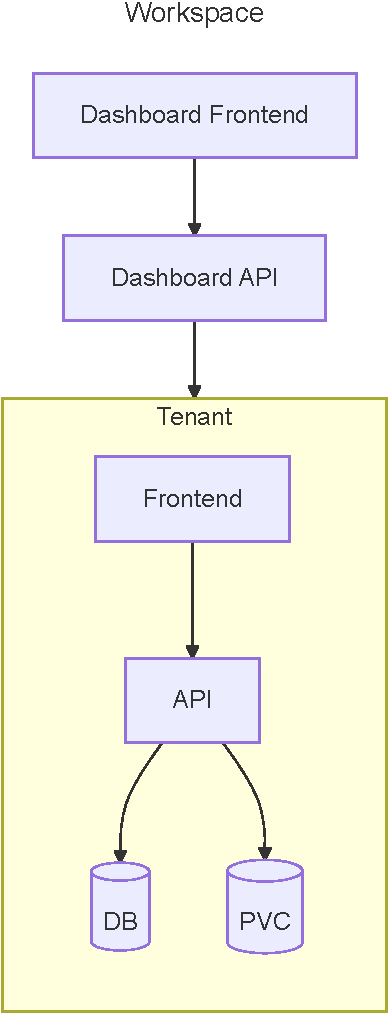
\includegraphics[scale=0.75]{images/WorkspaceArchitectureCropped.pdf}
                    \caption{Overview of the system architecture}\label{fig:system-architecture}
                \end{figure}

            \subsubsection{Rationale for Config Injection Strategy}\label{subsubsec:rationale}
                To enable tenant-specific customization in a secure and maintainable manner, the
                configuration is injected directly into the \gls{api} container during image build
                time using the \gls{docker} \texttt{--build-arg} mechanism.
                This approach ensures that the configuration resides fully within the corresponding
                tenant's workspace post-deployment, thereby preserving strong workspace isolation.
                Moreover, it avoids the operational complexity associated with runtime config
                injection mechanisms and simplifies the tenant lifecycle by keeping all relevant
                data embedded within the container image.
                \\
                Several alternative approaches were considered during the design process.
                Each of them was evaluated based on criteria such as workspace boundary isolation,
                persistence, scalability, operational complexity, and dependency footprint.
                The following list summarizes these alternatives and the primary reasons for their
                exclusion:

                \begin{enumerate}[label={[\arabic*]:},
                    ref=Challenge~\arabic*,
                    leftmargin=*,
                    itemsep=0.6\baselineskip]

                    \item\label{chal:pv}
                        \textit{\gls{pv}}.
                        \glspl{pv} offer cluster-wide storage, but they are bound to the
                        underlying infrastructure and not scoped to individual workspaces.
                        Since tenant data must remain fully isolated within its respective
                        workspace, using a shared \gls{pv} would have violated this design
                        constraint.
                        Furthermore \glspl{pv} would introduce significant operational complexity.
                        
                    \item\label{chal:pvc}
                        \textit{\gls{pvc}}.
                        \glspl{pvc} are workspace-scoped and technically suitable for storing tenant
                        configuration.
                        However, managing their lifecycle dynamically per tenant (including updates
                        and clean-up) would introduce significant operational complexity.

                    \item\label{chal:configMap}
                        \textit{ConfigMap}.
                        A ConfigMap is a lightweight and \gls{k8s} native way to inject
                        configuration, but it has a very constraining size limit (typically 1 MiB)
                        and is not designed for cross-workspace usage.  
                        Since KCP workspaces enforce strict isolation, injecting a ConfigMap from
                        the parent workspace into the tenant workspace would violate boundary
                        constraints, or require custom controllers.  
                        It was primarily not considered a viable long-term option due to its limited
                        support for binary data and poor scalability with growing or media-rich
                        configuration payloads.

                    \item\label{chal:gitRepo}
                        \textit{Git Repository}.
                        Polling or pulling tenant configuration from a Git repository would offer
                        central control and versioning, but would couple each tenant's runtime to an
                        external dependency.
                        It would also require embedding Git credentials or \gls{ssh} keys within the
                        workspace, raising security concerns and operational burden.
                        Furthermore the data does not live inside the tenant violating isolation
                        principles.

                    \item\label{chal:initContainer}
                        \textit{initContainer + emptyDir}.
                        This approach involves using an \texttt{initContainer} to write the config
                        into an \texttt{emptyDir} shared volume before the main \gls{api} container
                        starts.
                        While this ensures data locality, the config is ephemeral and lost on pod
                        restart or rescheduling.
                        Additionally, updates would require a full pod redeployment including
                        controlled init re-execution, adding complexity.

                    \item\label{chal:tenantDB}
                        \textit{Tenant \gls{db}}.
                        Storing the configuration in the tenant database would offer persistence and
                        locality.
                        However access control for the write operations and reaching out to the
                        \gls{db} from the parent workspace are critical pain points.

                    \item\label{chal:redis}
                        \textit{\gls{redis}}.
                        A Redis store within the tenant workspace was considered for fast config
                        access.
                        However, this introduces a full additional service dependency per tenant,
                        which contradicts the goals of lightweight and cost-efficient tenant
                        deployments.
                        Redis also requires persistence management if configuration must survive
                        restarts, therefore adding complexity.

                    \item\label{cahl:centralStore}
                        \textit{Central Document Store}
                        Maintaining a central document store in the root workspace (e.g. MongoDB or
                        MinIO) was ruled out due to isolation concerns.
                        This would require the tenant \gls{api} to reach out beyond its workspace
                        boundary, which is explicitly avoided in the current architecture to enforce
                        strict data sovereignty per tenant.
                \end{enumerate}

                Ultimately, the chosen build-time config injection strategy strikes an effective
                balance between strong tenant isolation, operational simplicity, and runtime
                performance.
                While it requires an image rebuild for every configuration change, this trade-off is
                acceptable given the infrequent update pattern of tenant configuration and the clear
                benefits it provides in terms of system architecture and security boundaries.
                \cleardoublepage

            \subsubsection{Data Synchronization and Caching Strategy}\label{syncAndCache}
                As the tenant-\gls{api} is built with its own \textbf{static} \texttt{config.json}
                as shown above \see{subsubsec:rationale}, the resulting caching strategy is
                straightforward.
                At startup the tenant-\gls{api} reads the immutable \texttt{config.json} that is
                baked into the container images \gls{fs}.
                Because the file never changes, while the image is running, the \gls{api} loads its
                content once, materializes the contents \textbf{in memory}, and attaches a single
                long-lived cache entry with a \gls{ttl} of 24~hours.
                A daily \gls{ttl} offers two advantages without introducing the complexity of an
                explicit cache invalidation.
                
                \begin{enumerate}[label={[\arabic*]:},
                    ref=Challenge~\arabic*,
                    leftmargin=*,
                    itemsep=0.6\baselineskip]

                    \item\label{chal:cachePerformance}
                        \textit{Performance}.
                        Subsequent requests bypass \gls{fs} \gls{io} entirely and are served from
                        memory, massively increasing speed and reducing disk pressure under burst
                        traffic.

                    \item\label{chal:cacheResilience}
                        \textit{Resilience and self-healing}.
                        Although the file is static, a bounded \gls{ttl} guarantees that each pod
                        refreshes its configuration once per day, so \textit{\gls{bitrot}} or a
                        silently corrupted memory page cannot persist indefinitely.
                        
                \end{enumerate}

                Because the only legitimate way to alter tenant configuration is to build and deploy
                a new image, a shorter \gls{ttl} or a manual cache-flush \gls{api} would add
                operational complexity without practical benefit.
                Caching the configuration with a long \gls{ttl} therefore strikes the best balance
                between maximal runtime throughput and the minimal housekeeping needed to keep every
                pod's view of configuration fresh and fault-tolerant over time.

            \subsubsection{Workspace Topology and Multi-Tenancy model}\label{subsubsec:workspaceTopology}

                % TODO: fix spacings
                \begin{table}[H]\label{tab:layersOverview}
                    \centering
                    \renewcommand{\arraystretch}{1.5}
                    \begin{tabular}{lcp{4cm}P{8cm}}
                        \toprule
                        Layer & \gls{kcp} construct & Example resources & Provisioned Amount \\
                        \midrule
                        Parent (control) & Workspace (\texttt{root}) & \texttt{dashboard}, \texttt{dashboard-api} Deployments & 1 (static) \\
                        Tenant (data) & Workspace (\texttt{root:<tenant-id>}) & \texttt{frontend}, \texttt{tenant-api} Deployments, \texttt{\gls{db}} StatefulSet & 1 per tenant \\
                        \bottomrule
                    \end{tabular}
                    \caption{Overview of architectural layers}
                \end{table}

                The system architecture is logically divided into two primary layers, a static
                parent workspace and a dynamically provisioned set of tenant workspaces.
                Each layer corresponds to a dedicated \gls{kcp} workspace and fulfills distinct
                responsibilities.
                \\
                The parent workspace acts as the control plane of the system.
                It hosts globally accessible resources such as the Dashboard frontend and the
                \gls{api} responsible for tenant lifecycle management.
                It exists as a single static \texttt{root} workspace and is not scaled horizontally.
                \\
                Each tenant is isolated in its own dedicated workspace (\texttt{root:<tenant-id>})
                created via \gls{kcp}'s Workspace \gls{crd} \gls{api}.
                These tenant workspaces are dynamically provisioned on demand through the
                \texttt{dashboard-\gls{api}}.
                They encapsulate all data and execution logic associated with the tenant, including
                the tenant-specific \gls{api}, frontend, and database state.
                \\
                Tenant workspaces are strictly isolated from each other and from the parent
                workspace.
                All tenant-related resources, including configuration and persistent state, reside
                exclusively within their respective workspaces, maintaining full logical and
                operational isolation.
                \\
                Deleting a workspace recursively tears down all associated Kubernetes resources,
                ensuring complete and automated cleanup without additional control-plane logic.
                \cleardoublepage

            \subsubsection{Tenant Workspace: Data Plane Components}
                
                % TODO: why scale based on cpu + qps

                \begin{table}[H]\label{tab:tenantComponents}
                    \centering
                    \renewcommand{\arraystretch}{1.5}
                    % TODO: fix spacings
                    \begin{tabular}{lp{4cm}P{8cm}}
                        \toprule
                        Component & Scaling & Purpose \\
                        \midrule
                        Frontend (\gls{next}) & \gls{hpa} based on \gls{cpu} and \gls{qps} & Serves static \gls{html} / \gls{js}, does \gls{ssr} for dynamic contents \\
                        \gls{api} (\gls{node}) & \gls{hpa} & Auth-less \gls{rest} endpoints with cache consumed by the \gls{next} app. \\
                        \gls{db} & StatefulSet & Stores ratings \\
                        \bottomrule
                    \end{tabular}
                    \caption{Per Tenant Components}
                \end{table}

                The request flow of the visitor path can be summarized as follows:

                \begin{enumerate}[label={[\arabic*]:},
                    ref=Challenge~\arabic*,
                    leftmargin=*,
                    itemsep=0.6\baselineskip]

                    \item\label{chal:frontend}
                        \textit{Frontend}.
                        The \gls{next} frontend is called.
                    \item\label{chal:tenantApi}
                        \textit{Tenant \gls{api}}.
                        The \gls{next} frontend calls the tenant \gls{api} to get dynamic data.
                        The tenant \gls{api} reads from the cache.

                    \item\label{chal:db}
                        \textit{Data sources}.
                        The tenant \gls{api} periodically renews its cache based of a \gls{ttl}.
                        The dynamic data (reviews) comes from the tenant \gls{db} while the static
                        data (config) comes from the tenant \gls{api}.
                \end{enumerate}

                This ensures, that for all customer interactions on the public website the workload
                remains local to the tenant workspace, thus improving the traceability.
            \subsubsection{Parent Workspace: Control Plane Components}\label{subsubsec:controlPlaneComponents}
                
                \begin{table}[H]\label{tab:parentComponents}
                    \centering
                    \renewcommand{\arraystretch}{1.5}
                    % TODO: fix spacings
                    \begin{tabular}{lp{4cm}P{8cm}}
                        \toprule
                        Component & Scaling & Purpose \\
                        \midrule
                        Dashboard & \gls{hpa} & Authenticated \gls{ui} for tenant owners; \gls{crud} operations on tenant data \\
                        Parent \gls{api} & \gls{hpa} & validates input and writes \gls{json} \\
                        \bottomrule
                    \end{tabular}
                    \caption{Control Plane Components}
                \end{table}

            \subsubsection{Scalability, Isolation and Security}\label{scalabilityIsolationSecurity}
                The described architecture should be able to provide a high level of scalability,
                isolation and security for the stated use case.
                It should achieve this as follows:

                \begin{enumerate}[label={[\arabic*]:},
                    ref=Challenge~\arabic*,
                    leftmargin=*,
                    itemsep=0.6\baselineskip]

                    \item\label{chal:architectureScalability}
                        \textit{Horizontal Scalability}.
                        Inside the tenant workspace the tenant-\gls{fe} and the tenant-\gls{api} run
                        as stateless deployments.
                        A \gls{hpa} driven by \gls{cpu} utilization and \gls{qps} metrics adds or
                        removes replicas linearly, so throughput increases proportionally with the
                        number of pods \see{tab:perTenantComponents}.
                        Because the \gls{api} keeps no local state, new replicas can be scheduled on
                        any node without coordination, ensuring that burst traffic on popular sites
                        never impacts neighboring tenants.

                    \item\label{chal:architectureIsolation}
                        \textit{Tenant Isolation}.
                        Every customer receives its ows dedicated \gls{kcp} workspace at onboarding
                        time.
                        A workspace maps to a private logical cluster stored in an independent
                        \gls{etcd} prefix, so objects created by one tenant are completely invisible
                        to others.
                        All runtime artifacts --- \gls{fe} pods, \gls{api} pods, \gls{db} and even
                        the \texttt{config.json} injected into the \gls{api} --- live exclusively
                        inside that workspace.
                        The platform never mounts cross-workspace volumes or reaches out to shared
                        data services.
                        Because there is \textbf{no shared state across workspaces} the design
                        should eliminate noisy-neighbor effects, simplify compliance and guarantee
                        data sovereignty for every tenant.

                    \item\label{chal:architectureSecurity}
                        \textit{Security}.
                        Multi-tenancy is only acceptable if confidentiality and integrity are
                        preserved across tenant boundaries.
                        \autoref{subsubsec:challenges} highlighted, that residual-data exposure,
                        cross-tenant access and side-channel attacks are the primary threats in
                        shared environments.
                        Because every tenant runs inside its \textbf{own} \gls{kcp} workspace,
                        backed by a private \gls{etcd} prefix, objects created in one workspace are
                        completely invisible to others, including non-namespaced objects like
                        \glspl{crd} \parencite{kcpWorkspaces}.
                        This hard logical boundary, combined with the absence of any shared state
                        outside the workspace allows for:
                        \\
                        \textbf{Data confidentiality}, as data resides inside the tenant,
                        eliminating residual-data exposure vectors.
                        \\
                        \textbf{Privilege containment}, as workspace-local \gls{rbac} rules grant
                        only verbs needed to operate intra-workspace resources and there are no
                        cluster-wide roles, blocking lateral movement and privilege-escalation
                        attempts.
                        \\
                        \textbf{Secure storage}, as only the tenant-\gls{api} has write access on
                        the tenant-\gls{db}.
                        \\
                        By confining a potential attacker to the compromised workspace, the
                        architecture should neutralize the multi-tenant security risks identified
                        earlier while still reaping the economic benefits of sharing the underlying
                        platform.
                        
                \end{enumerate}

                Collectively the security measures have to fulfill \hyperlink{NF-07}{nf7}.
                
                \cleardoublepage

        \subsection{Automated Deployment Strategies}\label{subsec:deploymentStrategies}
            Platform success depends on a deployment workflow that is fully automated, repeatable,
            and invisible to tenants.
            The design therefore distinguishes between the \textbf{first-time (initial) deployment}
            of a tenant workspace and the \textbf{continuous update policy} that keeps thousands of
            workspaces on a single, uniform release without interrupting production traffic.

            \subsubsection{Initial Tenant Deployment Pipeline}\label{subsubsec:initialDeeployment}
                When a new customer completes the on-boarding flow \hyperlink{f5}{F-05}, the
                Dashboard-\gls{api} running in the root workspace emits a custom resource
                (\texttt{TenantDeploymentRequest}) that seeds a GitOps pipeline
                (TODO: insert figure).
                The pipeline is implemented as a set of \textit{\gls{tekton}} tasks that run
                directly under the control of the Dashboard-\gls{api}, therefore no separate
                \textit{\gls{argocd}} controller is required.


                \begin{enumerate}[label={[\arabic*]:},
                    ref=Challenge~\arabic*,
                    leftmargin=*,
                    itemsep=0.6\baselineskip]

                    \item\label{chal:bootstrap}
                        \textit{Workspace bootstrap}.  
                        A controller watching for \texttt{TenantDeploymentRequest} objects
                        calls the \gls{kcp} \gls{api} to create a dedicated workspace
                        \texttt{root:\textless{}tenant-id\textgreater{}} and assigns only the
                        minimal \gls{rbac} roles required by the tenant components.


                    \item\label{chal:imageBuild}
                        \textit{Image build}.
                        A build task invokes \texttt{docker buildx} with
                        \texttt{--build-arg CONFIG\_JSON} to inject the tenant-specific
                        configuration into the \gls{api} image layer
                        (cf.~\autoref{subsubsec:rationale}).  
                        The resulting \gls{api} and \gls{fe} images are pushed to the internal
                        registry and tagged
                        \texttt{:\textless{}tenant-id\textgreater{}-\textless{}git-sha\textgreater{}}.

                    \item\label{chal:manifestRendering}
                        \textit{Manifest rendering}.
                        Helm/Kustomize templates are parameterized with the tenant ID, image
                        tags and a computed \texttt{ROUTE\_BASE} and rendered to plain \gls{yaml}.

                    \item\label{chal:routeAllocation}
                        \textit{Route allocation}.
                        The pipeline creates an \texttt{Ingress} (NGINX) or \texttt{Route}
                        (OpenShift) inside the tenant workspace.
                        A wildcard \gls{dns} entry (\texttt{*.example.com}) avoids central \gls{dns}
                        updates and keeps certificates simple.

                    \item\label{chal:applyManifests}
                        \textit{Deployment}.  
                        A Helm \texttt{upgrade --install} task applies the rendered manifests
                        in the tenant workspace, rolling out the \gls{fe}, \gls{api} and
                        backing \gls{db}.  
                        Readiness probes ensure the pipeline blocks until all Pods are ready.

                    \item\label{chal:callback}
                        \textit{Status callback}.  
                        Once every component is healthy, a final task POSTs the public \glspl{url}
                        and the image \gls{sha} back to the Dashboard-\gls{api}, which in turn marks
                        the tenant as \enquote{active} for subsequent logins.
                        
                \end{enumerate}

                By chaining these Tekton tasks the platform turns the single
                \texttt{TenantDeploymentRequest} event into a fully-isolated, routable tenant
                environment in one pass.
                Every artefact is generated from code that lives in Git, every cluster mutation is
                scoped to the tenant workspace, and every build is automatically signed by
                Tekton~Chains.
                Consequently the pipeline satisfies all functional requirements (TODO: which) while
                remaining short enough to version-control next to the product source and easy to
                extend with additional steps (e.g.\ quota enforcement or cost metering) as the
                service matures.

            \subsubsection{Continuous Deployment}\label{subsubsec:continuousDeployment}
                After the initial hand-off the platform must react to two kinds of change without
                operator intervention:

                \begin{enumerate}[label={[\arabic*]:},
                    ref=Challenge~\arabic*,
                    leftmargin=*,
                    itemsep=0.6\baselineskip]

                    \item\label{chal:cdCode}
                        \textit{Source-code updates}.
                        A merge on the main branch of either the tenant \gls{fe} or the tenant
                        \gls{api} Git repository emits a signed GitHub Webhook TODO: finish this
                        when more info is available
                        
                    \item\label{chal:cdData}
                        \textit{Content-driven updates (single tenant rebuild)}.
                        When business users change dynamic catalogue data or feature flags, the
                        dashboard \gls{api} issues a \texttt{TenantReconfigureRequest} object
                        that carries the new \texttt{config.json} payload.  
                        A dedicated Tekton pipeline in that tenant's workspace performs a rebuild of
                        the tenant \gls{api} image with a new \texttt{config.json}.
                        Following this a local helm upgrade of the tenant \gls{api} is performed,
                        while the \gls{fe} and \gls{db} remain untouched.

                \end{enumerate}

                \subsubsection{Zero-Downtime Rollout}\label{subsubsec:zeroDowntime}

                    Both continuous-deployment pipelines should deploy the updated version of the
                    tenant's application with zero downtime for customers while ensuring stability.
                    This can be achieved through a \textit{canary deployment}.
                    A canary deployment is a type of blue-green deployment strategy
                    \parencite[pp.~33--34]{awsOverviewDeploymentOptions}.
                    Blue-green deployments are a common deployment strategy to ensure zero downtime.
                    In a blue-green deployment the currently running application (blue) runs
                    alongside the newly deployed, updated application (green)
                    \parencite[pp.~32--33]{awsOverviewDeploymentOptions}[pp.~176--178]{davis2019}.
                    This allows for testing the green version in production, while still having the
                    blue version live to handle production traffic
                    \parencite[pp.~176--178]{davis2019}.
                    With a canary deployment, the cut-over from blue to green is performed
                    gradually \parencite[pp.~33--34]{awsOverviewDeploymentOptions}.
                    A small percentage of traffic is first routed to the green application,
                    the \textit{canary-group}, so that its real-world behavior can be observed under
                    production load \parencite[pp.~33--34]{awsOverviewDeploymentOptions}.
                    If no regressions are detected, the remaining traffic is shifted either in one
                    further step or through a series of linear increments until 100 \% of users are
                    served by the green version
                    \parencite[pp.~33--34]{awsOverviewDeploymentOptions}.
                    Because the blue environment remains intact throughout the process, any anomaly
                    can be mitigated instantly by redirecting requests back to it, thereby
                    minimizing blast radius while still achieving zero downtime for customers
                    \parencite[pp.~33--34]{awsOverviewDeploymentOptions}.
                    \\
                    Broken down step by step, the pipelines should act as follows:
                    
                    \begin{enumerate}[label={[\arabic*]:},
                        ref=Challenge~\arabic*,
                        leftmargin=*,
                        itemsep=0.6\baselineskip]

                        \item\label{chal:readinessProbe}
                            \textit{Readiness probe}.
                            Verifies readiness probes and functional smoke-tests on the green Pods.

                        \item\label{chal:shiftTraffic}.
                            \textit{Shift traffic}.
                            Shifts traffic incrementally by patching the weight on the tenant's
                            ingress.

                        \item\label{chal:canaryWindow}
                            \textit{Canary window}.
                            Aborts and rewinds the weight if any \gls{slo} breach or error-budget
                            drain is detected during the canary window.
                        
                        \item\label{chal:deletion}
                            \textit{Deletion}.
                            Deletes the blue deployment only after 100 \% of requests have
                            successfully moved to green.

                    \end{enumerate}

            \cleardoublepage

        \subsection{Choice of Technologies}\label{subsec:technologies}
            The platform architecture leverages modern, well-supported technologies that align with
            the core design principles of modularity, performance, and isolation.
            Each major component is built using tools selected for their suitability in a
            cloud-native, tenant-isolated SaaS environment.

            \begin{enumerate}[label={[\arabic*]:},
                ref=Challenge~\arabic*,
                leftmargin=*,
                itemsep=0.6\baselineskip]
                \item\label{chal:dashboardFE}
                    \textit{Dashboard \gls{fe}}.
                    The central Dashboard is implemented using \texttt{\gls{next}}.
                    Its file-based routing, support for both static and server-side rendering, and
                    seamless integration with TypeScript make it a suitable choice for building a
                    modular and responsive frontend.
                    Reusability and developer ergonomics were key factors in this decision.

                \item\label{chal:tenantFE}
                    \textit{Tenant \gls{fe}}.
                    Each tenant is provisioned with a separate frontend instance based on a shared
                    \texttt{\gls{next}} template.
                    This enables customization at the workspace level while maintaining consistent
                    structure and behavior.
                    \gls{next} also allows efficient static generation of tenant-specific content
                    during build time.
                    To further streamline provisioning, a pre-defined set of layout and component
                    \textit{skeletons} is embedded in the template repository.  
                    These skeletons provide a consistent structure for common views, while still
                    allowing per-tenant extension and branding.

                \item\label{chal:dashboardAPI}
                    \textit{Dashboard \gls{api}}.
                    The control plane's \gls{api} is built using \texttt{\gls{node}} and
                    \texttt{\gls{express}}, providing a lightweight, fast, and \gls{json}-native web
                    service environment.
                    It integrates a volatile \texttt{node-cache} layer for storing configuration
                    artifacts during tenant provisioning, minimizing external dependencies.

                \item\label{chal:tenantAPI}
                    \textit{Tenant \gls{api}}.
                    Each tenant workspace contains its own
                    \texttt{\gls{node}}~+~\texttt{\gls{express}} \gls{api} instance.
                    This ensures strict separation of runtime logic and supports injection of static
                    configuration at image build time.
                    The framework's flexibility and ecosystem make it well-suited for containerized
                    multi-tenant deployment.

                \item\label{chal:tempConfigStore}
                    \textit{Temporary Config Store}.
                    During tenant creation, configuration files are temporarily stored on the
                    Dashboard \gls{api}'s local filesystem.
                    These files are injected into the tenant image using Docker's
                    \texttt{--build-arg} and \texttt{COPY} mechanisms.
                    This avoids cross-workspace communication and external storage dependencies.

                \item\label{chal:tenantDB2}
                    \textit{Tenant \gls{db}}.
                    The tenants database layer is provided by \texttt{Citus}, a horizontally
                    scalable extension of PostgreSQL.\@
                    Citus allows sharded, isolated storage of tenant data and supports scaling out
                    as load increases.
                    Its compatibility with PostgreSQL clients simplifies development and
                    integration.

            \end{enumerate}

            This technology selection provides a robust foundation for implementing the desired
            multi-tenant \gls{saas} architecture while keeping the operational footprint minimal and
            the development process maintainable.
            Furthermore it aims to live inside the \gls{ts} ecosystem, simplifying the development
            process.
            \cleardoublepage

    \section{Prototypical Implementation}\label{sec:prototype}

        \subsection{Infrastructure with KCP}\label{subsec:infrastructure}

        \subsection[Tenant Provisioning]{Tenant Provisioning (Automation, Multi-Tenancy)}\label{subsec:tenantProvisioning}

        \subsection[Scaling Mechanisms]{Scaling Mechanisms (Horizontal Pod Autoscaler)}\label{subsec:scaling}
            \gls{hpa} in Kubernetes can react to any metric that the control plane exposes through
            resource or custom-metrics \glspl{api}.
            For a request-driven \textit{express} service, such as the tenant-\gls{api} the most
            accurate signal would be \textbf{\gls{qps}} at the ingress of each pod, because it
            tracks the real work performed and is immune to the noise that \gls{cpu}-bound metrics
            introduce when background jobs or garbage collection dominate a sample window.
            Nevertheless, the implementation in its prototypical nature deliberately relies on the
            built-in \textbf{\gls{cpu} utilization metric} alone, contrary to the architectural
            design.
            The choice is pragmatic rather than idealistic.
            Instrumenting per-pod \gls{qps} would require an extra metrics pipeline or at minimum a
            side-car that counts requests, a Prometheus deployment to scrape the counter, and a
            Prometheus adapter (or custom-metrics server) so the \gls{hpa} controller can consume
            the data.
            Each of those moving parts introduces significant configuration surface, security
            considerations, and potential failure modes that distract from the core objective of
            this thesis: to validate multi-tenant isolation and deployment strategies, not to
            engineer a production-grade observability stack.
            \gls{cpu} metrics, by contrast, are available out of the box from the kubelet and
            require only two declarative lines in the \gls{hpa} manifest.
            //
            Using \gls{cpu} as the scaling trigger therefore keeps the infrastructure lightweight,
            repeatable, and easy to grasp while still demonstrating that the platform can
            elastically adjust capacity under load.
            In a real-world \gls{saas} environment the \gls{hpa} spec could be refined to a compound
            metric using \gls{qps} latency percentiles, or custom business \glspl{kpi}, but for a
            prototype aimed at architectural proof of concept, the built-in metric is
            \enquote{good enough} and avoids adding too much complexity out of the thesis scope.

            \cleardoublepage

        \subsection[Monitoring and Logging]{Monitoring and Logging (Prometheus, Grafana)}\label{subsec:monitoring}

    \section{Evaluation}\label{sec:evaluation}

        \subsection[Performance Measurements]{Performance Measurements (Downtime, Latency, Scaling)}\label{subsec:performance}

        \subsection{Scaling Scenarios and Optimizations}\label{subsec:scalingOptimization}

        \subsection{Discussion of Results}\label{subsec:discussion}

    \section{Conclusion and Outlook}\label{sec:conclusion}

        \subsection{Summary}\label{subsec:summary}

        \subsection{Personal Conclusion}\label{subsec:personalConclusion}

        \subsection{Future Outlook}\label{subsec:outlook}

    \cleardoublepage
    \printbibliography[
        title = {References},
        heading = bibintoc
    ]

    \cleardoublepage
    \appendix

\end{document}
